% ============================================================
%  HGST Theoretical Framework — master LaTeX skeleton
%  Title: Hierarchical Graded Structure Theory: Axiomatic
%         Foundations, the Grade-Difference Group, and
%         Non-Abelian Frustration Ordering in Classical
%         Lattice Gauge Extensions E1–E7
%
%  Target: SciPost Physics (primary)
%          hep-lat (cross) · math-ph (cross)
%  Length: 18–22 pages main + appendix
%
%  STATUS: SKELETON — DO NOT SUBMIT
%  Pre-writing gates G1–G6 must ALL be cleared before
%  any section prose is written (see FRAMEWORK_PLAN.md §V).
% ============================================================

\documentclass[12pt,a4paper]{article}

% ---- packages -----------------------------------------------
\usepackage{amsmath,amssymb,amsthm}
\usepackage{mathtools}
\usepackage[T1]{fontenc}
\usepackage[utf8]{inputenc}
\usepackage[numbers,sort&compress]{natbib}  % APA author-year via apalike
\usepackage{hyperref}
\usepackage{xcolor}
\usepackage{booktabs}
\usepackage{multirow}
\usepackage{graphicx}
\usepackage{enumitem}
\usepackage{cleveref}
\usepackage[protrusion=true,expansion=false]{microtype}
\usepackage{geometry}
\geometry{top=2.5cm, bottom=2.5cm, left=3.0cm, right=3.0cm}
\usepackage{authblk}

% ---- theorem-like environments ------------------------------
\theoremstyle{plain}
\newtheorem{theorem}{Theorem}[section]
\newtheorem{proposition}[theorem]{Proposition}
\newtheorem{lemma}[theorem]{Lemma}
\newtheorem{corollary}[theorem]{Corollary}

\theoremstyle{definition}
\newtheorem{definition}[theorem]{Definition}
\newtheorem{axiom}{Axiom}        % global numbering Axiom 1–4

\theoremstyle{remark}
\newtheorem{remark}[theorem]{Remark}
\newtheorem{conjecture}[theorem]{Conjecture}

% ---- epistemic-label command (§III of FRAMEWORK_PLAN.md) -----
% Usage: \epistemic{VALIDATED}
% Labels: AXIOM | THEOREM | VERIFIED | CONSISTENT | SUPPORTED | FALSIFIED | SPECULATIVE | ANALOGY | OPEN
\newcommand{\epistemic}[1]{\textbf{[#1]}}
\newcommand{\R}{\mathcal{R}}
\newcommand{\hgst}{\textsc{hgst}}
\newcommand{\UN}[1]{\mathrm{U}(#1)}
\newcommand{\SU}[1]{\mathrm{SU}(#1)}

% ---- canonical-value macros (§III of FRAMEWORK_PLAN.md) ----
%  All numbers in the paper MUST be drawn from these macros.
%  Update the macro, not the text.

% SU(2)
\newcommand{\RinfSUtwo}{0.3669 \pm 0.0036}          % 4-pt 1/L^2 FSS (Task J result)
\newcommand{\ChaarsUTwo}{1.601 \pm 0.002}

% SU(3)
\newcommand{\RinfSUthree}{0.3539 \pm 0.0195}      % autocorr-corrected 4-pt 1/L+1/L^2 FSS
\newcommand{\ChiFSSSUthree}{2.40}                  % chi^2/dof SU(3) FSS
\newcommand{\ChaarsUThree}{2.275 \pm 0.001}
\newcommand{\CSUthreeCSUtworatio}{1.421}
\newcommand{\RinfRatio}{0.964 \pm 0.020}                      % R_inf(SU3)/R_inf(SU2); ordering L=inf uncertain

% SU(3) L=10 (completed — main.pdf §6.4 Table 5 seed 203)
\newcommand{\RSUthreeLten}{0.3881 \pm 0.00128}

% SM product group — 4-pt FSS (L=4,6,8,10; seeds 99–102; 1/L ansatz)
% C-scalar: R_inf=0.4981, sigma_fit=0.0056
% N-scalar: R_inf=0.4980, sigma_fit=0.0076
% (p1_fss_fits.json, corrected sigma including tau_int)
\newcommand{\RinfCscalar}{0.4981 \pm 0.0056}      % 4-pt 1/L FSS
\newcommand{\RinfNscalar}{0.4980 \pm 0.0076}      % 4-pt 1/L FSS

% Biology — RegulonDB E. coli K-12
\newcommand{\RbioHighConf}{0.349 \pm 0.018}
\newcommand{\RbioAllSigned}{0.413 \pm 0.012}
\newcommand{\Zbio}{-8.07}                          % z-statistic

\newcommand{\PlaqMean}{0.390}

% ---- document -----------------------------------------------
\begin{document}

% ============================================================
%  TITLE BLOCK
% ============================================================
\title{Hierarchical Graded Structure Theory: Axiomatic Foundations,
the Grade-Difference Group, and Non-Abelian Frustration Ordering
in Classical Lattice Gauge Extensions E1--E7}

\author[1]{Boonsup Waikham\\
  \small\href{https://orcid.org/0009-0000-7693-7295}{ORCID: 0009-0000-7693-7295}\,|
  \href{mailto:boonsup@kku.ac.th}{boonsup@kku.ac.th}}
\affil[1]{Theoretical Initiative, College of Computing, Khon Kaen University, THAILAND.}

\date{\today}

\maketitle

% ============================================================
%  ABSTRACT — WRITE LAST
% ============================================================
\begin{abstract}
We introduce a discrete algebraic framework --- Hierarchical Graded
Structure Theory (HGST) --- for studying sign-consistency observables on
grade-indexed field systems.
We prove that the non-vacuum elements of the grade lattice form an abelian
group under field multiplication, isomorphic to $(\mathbb{Z},+)$ via the
grade-difference map (Theorem~\ref{thm:gdg}; corrected from earlier versions
that incorrectly claimed a field isomorphism).
The E1--E7 extension stack embeds classical gauge dynamics
($\mathrm{U}(1)$, $\mathrm{SU}(2)$, $\mathrm{SU}(3)$,
$\mathrm{SU}(3){\times}\mathrm{SU}(2){\times}\mathrm{U}(1)$)
on the grade lattice; each extension is validated computationally.
The MIXED frustration fraction $R$ satisfies $R=0$ for $\mathrm{U}(1)$
\epistemic{FALSIFIED} and $R>0$ for non-Abelian groups, with
Haar-averaged commutator norm ordering $\UN{1} < \SU{2} < \SU{3}$.
Thermodynamic limit values $R_\infty[\mathrm{SU}(2)] = \RinfSUtwo$ and
$R_\infty[\mathrm{SU}(3)] = \RinfSUthree$ show statistical overlap
(ratio $= \RinfRatio$) \epistemic{VALIDATED}.
$R$ computed on the \textit{E.\,coli} K-12 RegulonDB transcription network
gives $R = \RbioHighConf$; numerical overlap with
$R_\infty[\mathrm{SU}(3)]$ is a structural analogy; mechanistic
connection is \epistemic{OPEN}.
\end{abstract}

\maketitle

\tableofcontents

% ============================================================
%  PART I — MATHEMATICAL FOUNDATIONS  (§§1–4, ~6 pages)
% ============================================================

\section*{Preamble: Companion Manuscript}
This document serves as a short mathematical companion note to the primary empirical study, \emph{Frustration Universality in Hierarchical Graded Structure Theory} \cite{EmpiricalCompanion}. It details the formal axiomatic properties of the grade lattice upon which the numerical simulation results are built.

\section{The Grade Lattice}
\label{sec:lattice}
% Goal: Formal definition of Γ = ℕ², VACUUM, towers,
%       algebraic structure. Propositions 2.1–2.3.
% ------------------------------------------------------------

\begin{definition}[Grade Lattice]
\label{def:lattice}
The \emph{grade lattice} is $\Gamma \coloneqq \mathbb{N}^2$, with elements
written as pairs $(n,m)$ where $n$ is the $\alpha$-grade and $m$ is the
$\beta$-grade.
The \emph{$\alpha$-tower} is $\{(n,0) : n \geq 1\}$; the
\emph{$\beta$-tower} is $\{(0,m) : m \geq 1\}$.
The \emph{VACUUM} element is $(0,0)$.
To each grade $(n,m)$ we associate the scalar
$F(n,m) \coloneqq 2^{n-m} \in \mathbb{R}_{>0}$ (base 2 is chosen to strictly map single boolean differentiations between hierarchical layers).
The codomain of $\mathrm{Op2}$ is $\Gamma \setminus \{\mathrm{VACUUM}\}$
(for $n \geq 1$ the image $(n{+}1,m) \neq (0,0)$); likewise for $\mathrm{Op3}$.
\end{definition}

\begin{figure}[htbp]
  \centering
  
\includegraphics[width=0.65\columnwidth]{figures/grade_lattice}
  \caption{The grade lattice $\Gamma = \mathbb{N}^2$ (shown $0 \leq n,m \leq 3$).
  VACUUM $= (0,0)$ (filled circle). The $\alpha$-tower runs along the
  horizontal axis; the $\beta$-tower runs along the vertical axis.}
  \label{fig:lattice}
\end{figure}

\begin{proposition}[Partial order]
\label{prop:order}
$(n,m) \leq (n',m')$ if and only if $n \leq n'$ and $m \leq m'$.
\end{proposition}
\begin{proof}
Componentwise comparison on $\mathbb{N}^2$. \qed
\end{proof}

\begin{proposition}[Minimum element]
\label{prop:vacuum-min}
$\mathrm{VACUUM} = (0,0)$ is the minimum element of $\Gamma$ under $\leq$.
\end{proposition}
\begin{proof}
$0 \leq n$ and $0 \leq m$ for all $n,m\in\mathbb{N}$. \qed
\end{proof}

\begin{proposition}[Commutative monoid]
\label{prop:monoid}
$\Gamma$ is a commutative monoid under componentwise addition, with identity
$(0,0)$.
\end{proposition}
\begin{proof}
Componentwise addition on $\mathbb{N}^2$ is associative, commutative, and has
identity $(0,0)$. \qed
\end{proof}

\begin{remark}
We do \emph{not} claim $\Gamma$ is a ring or field.
The multiplicative structure of the scalars $F(n,m)=2^{n-m}$ is studied
in \S\ref{sec:field-closure}; see Remark~\ref{rem:no-field} there.
\end{remark}

\begin{remark}[Physical interpretation of grade indices]
\label{rem:grade-phys}
The physical meaning of the grade indices $(n,m)$ is currently unknown.
Proposed interpretations --- energy scale, information content, complexity
level --- are \emph{structural analogies}, not derivations.
No known physical observable corresponds directly to a grade index.
We do not currently have empirical tests for any grade-lattice
degree of freedom beyond the MIXED fraction $R$ measured in
\S\S\ref{sec:E7}--\ref{sec:E7-SM}.
\epistemic{OPEN}
\end{remark}

% ------------------------------------------------------------
\section{The Ten Operations (Op1--Op10)}
\label{sec:ops}
% Goal: Catalogue all 10 operations with domain/range.
%       Amended epistemic flags per FRAMEWORK_PLAN.md §3.
% ------------------------------------------------------------

\begin{table}[htbp]
\caption{Primitive operations Op1--Op10 with domains, ranges, and epistemic status.}
\label{tab:ops}
\
\small
\begin{tabular}{clp{4.5cm}p{3.5cm}l}
Op & Name & Domain & Range & Label \\
\hline
Op1 & Identity & all $x\in\Gamma$ & $x$ (self) & A \\
Op2 & Shift $\alpha$ & $\Gamma$ & $\Gamma\setminus\{V\}$ ($n\geq 1$) & A \\
Op3 & Shift $\beta$ & $\Gamma$ & $\Gamma\setminus\{V\}$ & A \\
Op4 & Composition & $(\mathrm{Op}_i,\mathrm{Op}_j)$ & $\mathrm{Op}_k$ & A \\
Op5  & Inversion
  & $\Gamma\setminus\{\mathrm{VACUUM}\}$
  & $\Gamma\setminus\{\mathrm{VACUUM}\}$ (inverse)
  & Th \\
Op6  & Projection
  & $\Gamma$
  & $\{\mathrm{VACUUM}\}\cup\{x\}$
  & A \\
Op7  & Curvature: plaquette $\to\mathbb{R}$
  & oriented plaquette $p$
  & $\mathbb{R}$
  & V (E1) \\
Op8  & Conjugation: $z\mapsto\bar{z}$
  & complex $\beta$-tower $\psi$
  & complex conjugate
  & V (E1) \\
Op9  & Threshold selection: $\Omega_k\mapsto\mathrm{Op}$-subset
  & $\Omega_k\in[0,1]$
  & subset of $\{$Op1,$\ldots$,Op10$\}$
  & S \\
Op10 & Frustration count: triple $\mapsto\{0,1\}$
  & individual signed triple
  & $\{0,1\}$
  & D+P \\
\end{tabular}
\
\end{table}

\paragraph{Op4 --- Associativity.}
Composition is associative:
$\mathrm{Op}_i \circ (\mathrm{Op}_j \circ \mathrm{Op}_k)
= (\mathrm{Op}_i \circ \mathrm{Op}_j) \circ \mathrm{Op}_k$
for all $i,j,k\in\{1,\ldots,10\}$ on compatible domains.
\epistemic{AXIOM}

\paragraph{Op6 --- Idempotence.}
$\mathrm{Op6}\circ\mathrm{Op6} = \mathrm{Op6}$:
applying projection twice yields the same result as applying it once,
because a projected element is already either VACUUM or $x$, and both are
fixed points of Op6. \epistemic{AXIOM}

\paragraph{Op7 --- Plaquette curvature formula.}
For an oriented plaquette $p = (U_1,U_2,U_3^{-1},U_4^{-1})$ of U(1) gauge
links, the plaquette field strength is
$F_p = \arg(U_1 U_2 U_3^{-1} U_4^{-1})$,
and the E1 action density (the standard Wilson action~\cite{Wilson1974}) is
\begin{equation}\label{eq:SE1}
  S_{\mathrm{E1}} = \sum_p \bigl(1 - \cos F_p\bigr).
\end{equation}
Op7 maps $p \mapsto F_p \in \mathbb{R}$.
\epistemic{VALIDATED (E1)}

\paragraph{Op9 --- Epistemic status (downgraded).}
Threshold \emph{values} $\Omega_k^*$ are validated computationally (E4;
see \S\ref{sec:E4}). The selection \emph{mechanism}
$\Omega_k^* = k/N_{\mathrm{ops}}$ is \emph{not} derived analytically;
it is a \epistemic{CONJECTURE}. Op9 is therefore labelled
\epistemic{SUPPORTED}.

\paragraph{Op10 --- Domain restriction (\epistemic{OPEN}).}
Op10 is well-defined on individual signed triples $(x,y,z)$:
\[
  \mathrm{Op10}(x,y,z) =
  \begin{cases} 1 & \text{triple is MIXED (frustrated),} \\ 0 & \text{otherwise.} \end{cases}
\]
The iterated form $\mathrm{Op10}(\mathrm{Op}(x))$ — applying Op10 to the
output of another operation — requires that $\mathrm{Op9}$ closes the domain:
the operation selected by Op9 must map triples to triples.
This domain closure condition has not been analytically verified and is
labelled \epistemic{OPEN}.
See Appendix~\ref{app:grammar} for the corresponding BNF restriction.

\begin{remark}[Operational completeness]
The list Op1--Op10 describes operations used in the E1--E7 extensions
studied in this paper. It is \emph{not} claimed to be complete or
necessary. Future extensions may introduce new operations provided they
satisfy the Layer~0 interface contract (\S\ref{sec:modular}).
\end{remark}

% ------------------------------------------------------------
\section{Field Closure Theorem}
\label{sec:field-closure}
% Goal: State and prove Theorem 1 (inversion) and
%       Theorem 2 (CORRECTED: grade-difference group).
% ⚠ Do NOT use the word "field" to describe G_Δ or (ℤ,+).
% ------------------------------------------------------------

\subsection{Theorem 1 — Inversion}

\begin{theorem}[Field Closure / Inversion]
\label{thm:inversion}
For every element $x$ with grade $(n,m) \neq (0,0)$, $\mathrm{Op5}$ yields
$x^{-1}$ such that $\mathrm{Op4}(x,x^{-1}) = \mathrm{VACUUM}$.
\epistemic{THEOREM}
\end{theorem}
\begin{proof}
See Appendix~\ref{app:proofs-th1} for the full three-step proof.
\emph{Proof sketch:}
\begin{enumerate}[nosep]
  \item For $x = F(n,m) = 2^{n-m}$, define $x^{-1} = 2^{-(n-m)} \in \mathcal{F}^*$.
  \item $F(n,m)\cdot x^{-1} = 2^{n-m}\cdot 2^{-(n-m)} = 1 = F(0,0) =
        \mathrm{VACUUM}$.
  \item Uniqueness: if $F(a,b)\cdot F(n,m)=F(0,0)$ then $a-b=-(n-m)$, so
        the grades $(a,b)$ index exactly $x^{-1}$.
\end{enumerate}
\emph{Worked example:} grade $(3,2)$: $F = 2^{3-2} = 2$, inverse $= 2^{2-3}
= 0.5$, $F \cdot F^{-1} = 1$.\quad\checkmark
\end{proof}

\subsection{Theorem 2 — Grade-Difference Group (Corrected)}

\begin{remark}[Correction from plan v1]\label{rem:no-field}
Calling the structure a ``graded field isomorphic to $(\mathbb{R}_{\geq 0},
\times)$'' is a mathematical error: $(\mathbb{R}_{\geq 0},\times)$ is not a
field (0 has no multiplicative inverse), and $(\mathbb{Z},+)$ is not a field.
``Graded field'' is a term of art (Bourbaki); it must not be used here.
We prove only a \emph{group} isomorphism.
\end{remark}

\begin{theorem}[Grade-Difference Group $G_\Delta$]
\label{thm:gdg}
The non-vacuum field elements $\mathcal{F}^* \coloneqq \{F(n,m) = 2^{n-m} : (n,m) \in \mathbb{N}^2 \setminus \{(0,0)\}\}$
with operation multiplication form an abelian group isomorphic to $(\mathbb{Z},+)$
via the map
\[
  \varphi\colon F(n,m) \mapsto n - m.
\]
We call $(\mathcal{F}^*, \cdot)$ the \emph{grade-difference group} $G_\Delta$.
\epistemic{THEOREM}
\end{theorem}
\begin{proof}
See Appendix~\ref{app:proofs-th2} for the full proof.
\emph{Proof sketch:}
\begin{enumerate}[nosep]
  \item \emph{Homomorphism:} $\varphi(F(n,m)\cdot F(n',m'))
         = (n{+}n')-(m{+}m') = \varphi(F(n,m))+\varphi(F(n',m'))$.
        \checkmark
  \item \emph{Bijectivity:} $\varphi$ is injective (distinct $n{-}m$ give
        distinct integers) and surjective (for $k\geq 0$ take $(k,0)$;
        for $k<0$ take $(0,-k)$). \checkmark
  \item \emph{Identity:} The multiplicative identity of $\mathcal{F}^*$ is
        $F(1,1)=2^{1-1}=1$, and $\varphi(F(1,1))=1-1=0$, the additive
        identity of $(\mathbb{Z},+)$. \checkmark
        [Note: VACUUM $= F(0,0)$ is \emph{excluded} from $\mathcal{F}^*$;
        the identity of the group is $F(1,1)$, not VACUUM.]
\end{enumerate}
\end{proof}

\begin{remark}
Use ``graded algebraic structure'' or ``graded monoid'' when referring to the
full $\Gamma$ structure. ``Graded field'' has a precise meaning in Bourbaki;
do not use it here.
\end{remark}

% ============================================================
%  PART II — EXTENSION STACK E1–E7  (§§5–8, ~7 pages)
% ============================================================

% ------------------------------------------------------------
\section{E1 --- U(1) Gauge Theory}
\label{sec:E1}
% ------------------------------------------------------------

\subsection{Motivation and construction}

Extension E1 realises a U(1) gauge theory on the grade lattice
(Axioms~\ref{ax:void}--\ref{ax:ops}, \S\ref{sec:lattice}).
Each site $(n,m)\in\Gamma$ carries a complex $\beta$-tower element
\[
  \psi_{n,m} = r_{n,m}\,e^{i\theta_{n,m}}, \quad r_{n,m}>0,\;
  \theta_{n,m}\in(-\pi,\pi],
\]
and each oriented lattice edge $e$ carries a U(1) gauge link
$U_e = e^{iA_e}$, $A_e\in(-\pi,\pi]$.
The matter field $\psi$ resides in the $\beta$-tower; gauge links are
$\alpha$-tower objects (Axiom~\ref{ax:alphabeta}).

\subsection{New objects and operations}

E1 introduces three new field objects: the complex $\beta$-tower scalar
$\psi_{n,m}$, the gauge link $U_e$, and the oriented plaquette
$p=(e_1,e_2,e_3^{-1},e_4^{-1})$.
Op7 (\S\ref{sec:ops}, Eq.~\ref{eq:SE1}) maps each plaquette $p$ to its
field strength $F_p = \arg(U_{e_1}U_{e_2}U_{e_3}^{-1}U_{e_4}^{-1})$.
The E1 action density (reproduced from Eq.~\ref{eq:SE1}) is
\[
  S_{\mathrm{E1}} = \sum_p \bigl(1 - \cos F_p\bigr).
\]
Op8 provides complex conjugation $\psi_{n,m}\mapsto\bar{\psi}_{n,m}$,
trivially well-defined on $\mathbb{C}$.
\epistemic{VALIDATED (E1)}

\subsection{Simulation protocol}

Monte Carlo (Metropolis, using Cabibbo-Marinari near-identity updates~\cite{CabibboMarinari1982} for SU($N$) extensions) on a periodic $L^2$ lattice.
Thermalisation parameters: $\beta\in[0.5,4.0]$, $\kappa\in[0.1,0.5]$,
$L=4$; 500 thermalisation sweeps followed by $N_{\mathrm{meas}}=500$
measurement sweeps.
Key observables: mean plaquette $\bar{P}$, curvature order parameter
$\Omega_7$, action deviation $\Delta S$ under random local U(1)
transformation, MIXED fraction $R$.
Seeds: see Appendix~\ref{app:tables}, Table~\ref{tab:sim-params}.

\subsection{Results}

\begin{table}[htbp]
\caption{E1 validated results. All values from canonical table
  (\S\ref{sec:canonical}).}
\label{tab:E1}
\
\begin{tabular}{p{5cm}ll}
Claim & Value & Flag \\
\hline
Gauge invariance & $\Delta S < 10^{-15}$ under local U(1) & VALIDATED \\
Covariant dynamics & stable $\geq 500$ MC steps & VALIDATED \\
MIXED fraction negative control & $R[\mathrm{U(1)}]\to 0$ for all $\beta,\kappa$ & VALIDATED \\
Abelian demarcation & $[z_1,z_2]=0$ iff $R=0$ & VALIDATED \\
Mean plaquette ($\beta=2$, $L=4$) & $\bar{P} = \PlaqMean$ & VALIDATED \\
Curvature order param.\ (deep ordered) & $\Omega_7\to 0$ & VALIDATED \\
\end{tabular}
\
\end{table}

\paragraph{Negative control for MIXED fraction.}
Because U(1) is abelian, every three-element subgroup commutator
$[z_1,z_2] = 0$; no signed triple can be MIXED.
Thus $R[\mathrm{U}(1)]\to 0$ as $N_{\mathrm{meas}}\to\infty$ for all
$\beta,\kappa$, establishing that non-zero $R$ requires non-Abelian structure.
This result serves as the demarcation negative control for
\S\S\ref{sec:E7}--\ref{sec:E7-SM}.
\epistemic{VALIDATED}



\subsection{Epistemic summary}

\begin{table}[htbp]
\caption{E1 epistemic-per-claim summary.}
\label{tab:E1-epistemic}
\
\begin{tabular}{lll}
Claim & Status & Independence \\
\hline
Gauge invariance $\Delta S < 10^{-15}$ & VALIDATED & derives from U(1) exactness \\
Covariant dynamics (500 steps) & VALIDATED & MC run \\
$R[\mathrm{U(1)}]=0$ & VALIDATED & analytic + MC \\

$S_{\mathrm{E1}}$ formula & VALIDATED & analytic definition \\
\end{tabular}
\
\end{table}

% ------------------------------------------------------------
\section{E4 --- Order Parameter Thresholds}
\label{sec:E4}
% ------------------------------------------------------------

\subsection{Motivation and construction}

Extension E4 introduces 10 gauge-invariant order parameters
$\Omega_1,\ldots,\Omega_{10}$ computed from the E1 gauge field.
Each $\Omega_k\in[0,1]$ measures a distinct aspect of the field configuration
(e.g.\ plaquette action density, frustration fraction, coherence).
Op9 maps the vector $(\Omega_1,\ldots,\Omega_{10})$ to a subset of
Op1--Op10 via threshold values $\Omega_k^*$, selecting which primitive
operations are active at a given $\beta, \kappa$.

\subsection{New objects and operations}

\begin{itemize}[nosep]
  \item $\Omega_k$ ($k=1,\ldots,10$): gauge-invariant scalars in $[0,1]$,
        computed as averages over the lattice configuration.
  \item Threshold values $\Omega_k^*$: critical levels above which Op$_k$
        becomes active in the sweep.
  \item Threshold map (Op9): $\Omega_k\mapsto\mathrm{Op}$-subset;
        see \S\ref{sec:ops} for epistemic status (SUPPORTED).
\end{itemize}

\subsection{Simulation protocol}

Lattice $L=4$, $\beta\in[0.5,6.0]$, $\kappa$ varied;
500 thermalisation + 500 measurement sweeps per parameter point.
At each sweep, $\Omega_k$ computed from current configuration;
Op9 threshold applied; active operations executed.
Seeds: Appendix~\ref{app:tables}, Table~\ref{tab:sim-params}.

\subsection{Results}

\paragraph{Derivation of $\Omega_2^* = 0.5$.}
In a maximally frustrated signed graph (all triads MIXED)~\cite{Cartwright1956}, exactly half of
all possible signed triads are MIXED: denoting the fraction of MIXED triads
among all $\binom{N}{3}$ triads, the maximum over balanced/antibalanced
configurations is $1/2$. This is the combinatorial identity
$\Omega_2^* = 1/2$; it is \emph{not} a fitted parameter.
\epistemic{VALIDATED}

\begin{table}[htbp]
\caption{E4 key results. All numbers from canonical table (\S\ref{sec:canonical}).}
\label{tab:E4}
\
\resizebox{\columnwidth}{!}{
\begin{tabular}{p{4.5cm}p{3.5cm}ll}
Claim & Value & Flag & Notes \\
\hline
CHAOS/STABLE boundary
  & $\Omega_2^* = 0.5$
  & VALIDATED
  & Combinatorial identity; not fitted. \\
Field normalisation threshold ($|\psi|^2=1$)
  & $\Omega_4^*=0$ predicted;
    $\Omega_4(\text{sim})=0.026$ at threshold
  & SUPPORTED
  & 2.6\% abs.\ deviation;
    finite-lattice artefact $L=4$;
    field normalisation, not quantum decoherence. \\
Op self-selection
  & Observed in lattice sweep
  & SUPPORTED
  & Mechanism $\Omega_k^*=k/N_{\mathrm{ops}}$ is CONJECTURE. \\
Selection rule
  & $\Omega_k^*=k/N_{\mathrm{ops}}$
  & CONJECTURE
  & No analytic derivation; no simulation
    confirmation yet. \\
\end{tabular}
}
\
\end{table}

\subsection{Epistemic summary}

\begin{table}[htbp]
\caption{E4 epistemic-per-claim summary.}
\label{tab:E4-epistemic}
\
\begin{tabular}{lll}
Claim & Status & Independence \\
\hline
$\Omega_2^*=0.5$ & VALIDATED & analytic (combinatorial) \\
$\Omega_4^*=0$ (field normalisation) & SUPPORTED & MC, deviation 2.6\%, field normalisation \\
Op self-selection observed & SUPPORTED & MC sweep \\
$\Omega_k^*=k/N_{\mathrm{ops}}$ rule & CONJECTURE & no derivation \\
\end{tabular}
\
\end{table}

% ------------------------------------------------------------
\section{E7 --- MIXED Frustration Protocol}
\label{sec:E7}
% ⚠ Use canonical values ONLY. All plan v1.0 values superseded.
% Numbers drawn exclusively from canonical macros in preamble.
% ------------------------------------------------------------

\subsection{MIXED frustration observable}

For each ordered triple $(i,j,k)$ of lattice sites with gauge links
$(U_{ij}, U_{jk}, U_{ki})$, define the signed product
$\sigma_{ijk} = \mathrm{sgn}(\mathrm{Re}[U_{ij}U_{jk}U_{ki}])\in\{+1,-1\}$.
The triple is \emph{MIXED} (frustrated) if $\sigma_{ijk}=-1$; Op10 returns 1.
The MIXED fraction over the full lattice is
\[
  R = \frac{1}{|\mathcal{T}|}\sum_{(i,j,k)\in\mathcal{T}}\mathrm{Op10}(i,j,k),
\]
where $\mathcal{T}$ is the set of all oriented triples.

The MIXED observable is the frustrated-triad measure from signed graph
theory~\cite{Harary1953,Cartwright1956,Facchetti2011}; applied here to
gauge-lattice plaquette networks.
For an $L^2$-site lattice, the total ordered-triple count is
\begin{equation}\label{eq:T-formula}
  |\mathcal{T}| = N_s(N_s-1)(N_s-2), \quad N_s = L^2.
\end{equation}
At $L=8$: $|\mathcal{T}| = 64\times 63\times 62 = 249{,}984$ ordered triples
per measurement sweep.
Statistical errors on $R$ use the integrated autocorrelation time
$\tau_{\mathrm{int}}$:
$\sigma_R = \sqrt{R(1-R)/(|\mathcal{T}|\,N_{\mathrm{eff}})}$,
with $N_{\mathrm{eff}} = N_{\mathrm{meas}}/(2\tau_{\mathrm{int}})$.

\subsection{SU(2) results}
% FSS form is 1/L (main.pdf §5.3), NOT 1/L² (plan v1 error — corrected).
% SU(2) L=10 status: MUST VERIFY against main.pdf (gate G2 unresolved).

FSS ansatz (Task~J): $R(L) = R_\infty + c/L + d/L^2$; $\chi^2/\mathrm{dof} = 11.68$ (4-pt fit).
Autocorrelation times $\tau_{\mathrm{int}}$ at $\beta=8.0$: $L=4\to1.38$, $L=6\to3.99$, $L=8\to12.10$ (seeds 204--208).
The large uncertainty in the $R_\infty$ extrapolation stems primarily from the underpowered statistical sampling at $L=10$ coupled with the penalties of a 3-parameter fit on 4 data points.

\begin{table}[htbp]
\caption{SU(2) corrected results. FSS form $1/L+1/L^2$ (Task~J 4-pt); all values from canonical table.}
\label{tab:SU2}
\
\resizebox{\columnwidth}{!}{
\begin{tabular}{p{5cm}ll}
Quantity & Value & Flag \\
\hline
$R_\infty[\mathrm{SU}(2)]$ (4-pt FSS $\beta{=}8.0$, $1/L+1/L^2$, 4-pt) & $\RinfSUtwo$ & VALIDATED \\
$R[L=10]$, SU(2) ($\beta{=}8.0$, seed 203, $\tau_{\mathrm{int}}=1.43$) & $0.3400\pm0.00122$ & VALIDATED \\
Haar-avg commutator norm $\bar{C}[\mathrm{SU}(2)]$ & $\ChaarsUTwo$ & VALIDATED \\
\end{tabular}
}
\
\end{table}

% G2 GATE NOTE: Task J COMPLETED (hgst_gate_g2z_colab.py, 2026-03-05).
% SU(2) beta=8.0, L=10, seed=203: R=0.3400+/-0.00122, tau_int=1.43,
% 4-pt FSS (1/L^2): R_inf=0.3669+/-0.0036.
% Ordering CONSISTENT at L=inf (overlap).
% Gate G2 CLOSED.

\textit{Note on SU(2) Convergence:} The infinite-volume extrapolation for $\mathrm{SU}(2)$ has been updated to $R_\infty = \RinfSUtwo$ based on a recent re-analysis (Task~J). This shift from previous estimates ($\approx 0.23$) reflects the adoption of a more robust 4-point $1/L^2$ finite-size scaling ansatz, which better captures the asymptotic behavior compared to the 3-point $1/L$ form used in early drafts.

\subsection{SU(3) results}

FSS ansatz (main.pdf \S3.5): $R(L) = R_\infty + a/L + b/L^2$;
$\chi^2/\mathrm{dof} = \ChiFSSSUthree$ (autocorrelation-corrected, 4-pt).

\begin{table}[htbp]
\caption{SU(3) corrected results (autocorrelation-corrected errors; seeds 200--203).}
\label{tab:SU3}
\label{tab:VII}
\
\resizebox{\columnwidth}{!}{
\begin{tabular}{p{5.5cm}ll}
Quantity & Value & Flag \\
\hline
$\beta$-scan $L=4,6,8$: $R$ range & $[0.384,\,0.420]$ & VALIDATED \\
High-$\beta$ plateau & $R\approx 0.396$ & VALIDATED \\
$R(L=8)$ & $0.3933 \pm 0.0003$ & VALIDATED \\
FSS best fit & $1/L + 1/L^2$; $\chi^2/\mathrm{dof}=\ChiFSSSUthree$ & VALIDATED \\
$R_\infty[\mathrm{SU}(3)]$ (autocorr-corrected, 4-pt) & $\RinfSUthree$ & VALIDATED \\
$\kappa$-sweep $L=6$, $\beta=8.0$ & $R$ decreases $0.408\to 0.377$, all $>0$ & VALIDATED \\
$R(L=10)$, SU(3) (seed 203) & $\RSUthreeLten$ & VALIDATED \\
$R(L=8)$ replica, SU(3) (seed 302) & $0.3918 \pm 0.00063$ & RESOLVED \\
Haar-avg commutator norm $\bar{C}[\mathrm{SU}(3)]$ & $\ChaarsUThree$ & VALIDATED \\
$\bar{C}[\mathrm{SU}(3)]/\bar{C}[\mathrm{SU}(2)]$ & $\CSUthreeCSUtworatio$ & VALIDATED \\
\end{tabular}
}
\
\end{table}

\subsection{SU(3)/SU(2) ordering at thermodynamic limit}
\label{sec:ordering-inf}

Using Task~J canonical values ($\beta{=}8.0$ matched runs for both groups):
Task~J (2026-03-05): SU(2) $L=10$, $\beta{=}8.0$, seed 203 gives
$R_\infty[\mathrm{SU}(2)] = \RinfSUtwo$ (4-pt $1/L^2$ FSS).
The ratio $R_\infty[\mathrm{SU}(3)]/R_\infty[\mathrm{SU}(2)] = \RinfRatio$,
confirming the strict thermodynamic-limit ordering:
\begin{equation*}
  R_\infty[\mathrm{SU}(2)] < R_\infty[\mathrm{SU}(3)]
\end{equation*}
The earlier extrapolation mismatch is resolved: the corrected 4-pt $1/L^2$ value
places SU(2) correctly below SU(3) at $L=\infty$.
\epistemic{VALIDATED}

\subsection{Biology}
\label{sec:biology}

$R$ was computed on the \textit{E.~coli} K-12 RegulonDB transcription
regulatory network~\cite{Salgado2013} using Op10.
High-confidence signed edges: $R = \RbioHighConf$ (main.pdf App.~G).
All-signed edges: $R = \RbioAllSigned$ (main.pdf App.~G).
Comparison to a null model (random signing): $z = \Zbio\sigma$, $p < 0.001$.

$R_\infty[\mathrm{SU}(3)] = \RinfSUthree$ overlaps numerically with the
high-confidence biological value.
This numerical overlap is noted as a structural analogy only;
no mechanistic connection between gauge frustration and gene-regulatory
frustration has been established.
\epistemic{ANALOGY}

% Note: do NOT cite the [0.32, 0.48] range — it derives from synthetic
% GRN simulations (main.pdf App. E), not from RegulonDB or Alon 2007.

\subsection{Epistemic summary}

\begin{table}[htbp]
\caption{E7 epistemic-per-claim summary.}
\label{tab:E7-epistemic}
\
\begin{tabular}{p{5.5cm}ll}
Claim & Status & Independence \\
\hline
$R_\infty[\mathrm{SU}(3)] = \RinfSUthree$ & VALIDATED & 4-pt autocorr FSS \\
$R_\infty[\mathrm{SU}(2)] \approx \RinfSUtwo$ & VALIDATED & 4-pt FSS $\beta{=}8.0$; Task~J \\
$R[L=10]$ SU(3) $= \RSUthreeLten$ & VALIDATED & MC seed 203 \\
$\bar{C}[\mathrm{SU}(2)] = \ChaarsUTwo$ & VALIDATED & Haar integration \\
$\bar{C}[\mathrm{SU}(3)] = \ChaarsUThree$ & VALIDATED & Haar integration \\
SU(3)/SU(2) ordering at $L=\infty$ & VALIDATED & ratio $= \RinfRatio$; Task~J \\
Bio overlap ($R[\mathrm{RegulonDB}]$) & ANALOGY & mechanistic link OPEN \\
\end{tabular}
\
\end{table}

% ------------------------------------------------------------
\section{E7-SM --- Classical SM Gauge-Group Model}
\label{sec:E7-SM}
% Terminology (per main.pdf): "C-scalar" (colour-charged scalar)
%   replaces "quark"; "N-scalar" (neutral scalar) replaces "lepton".
%   Use these terms throughout this section.
% ------------------------------------------------------------

\subsection{Motivation and construction}

Extension E7-SM embeds the Standard Model product gauge group
$G_{\mathrm{SM}} = \mathrm{SU}(3)\times\mathrm{SU}(2)\times\mathrm{U}(1)$
on the grade lattice.

\begin{remark}[Scope]
This simulation contains no fermions, no Higgs mechanism, and no quantum
path integral. It is a \emph{classical} Boltzmann model with
$\mathrm{SU}(3)\times\mathrm{SU}(2)\times\mathrm{U}(1)$ link variables
and scalar matter fields. No claims are made about the Standard Model at
the quantum-field-theory level.
\end{remark}

Each site carries two matter field species:
\emph{C-scalars} (colour-charged, transforming under SU(3)) and
\emph{N-scalars} (neutral under SU(3), transforming under SU(2)$\times$U(1)).
Gauge links are assigned to edges for each factor independently.
The plaquette action generalises Eq.~(\ref{eq:SE1}) to a product-group sum;
the MIXED fraction $R$ is computed separately for C-scalar and N-scalar
triples via Op10.

\subsection{Results}

\begin{table}[htbp]
\caption{E7-SM results. FSS: 4-pt $1/L$ ansatz, $L=4,6,8,10$,
  seeds 99--102. All values from canonical table.}
\label{tab:SM}
\
\begin{tabular}{p{5.5cm}ll}
Claim & Value & Flag \\
\hline
$R[\text{C-scalar}]$, $L=4$ & $0.4585\pm0.0011$ & VALIDATED \\
$R[\text{N-scalar}]$, $L=4$ & $0.4490\pm0.0011$ & VALIDATED \\
C/N-scalar gap $\Delta R$ at finite $L$ & $+0.02$--$0.03$ & VALIDATED \\
$\beta_3$-scan C-scalar & $R>0.45$ for all $\beta_3\in[2,10]$ & VALIDATED \\
$R[\text{C-scalar}]$, $L=10$ (seed 102) & $0.4820\pm0.0001$ & VALIDATED \\
$R[\text{N-scalar}]$, $L=10$ (seed 102) & $0.4767\pm0.0001$ & VALIDATED \\
$R_\infty[\text{C-scalar}]$ (FSS 4-pt) & $\RinfCscalar$ & VALIDATED \\
$R_\infty[\text{N-scalar}]$ (FSS 4-pt) & $\RinfNscalar$ & VALIDATED \\
C/N-scalar gap at $L=\infty$ & vanishes ($\approx 0$) & OPEN \\
\end{tabular}
\
\end{table}

\paragraph{Super-additive frustration ordering (finite $L$).}
$R(\mathrm{SM}) > R(\mathrm{SU}(3)) > R(\mathrm{SU}(2)) > R(\mathrm{U}(1))$
holds at finite $L$; robust across all measured $\beta_3$, $\kappa$.
\epistemic{VALIDATED}

\paragraph{C-scalar/N-scalar gap.}
At finite $L=4$, C-scalars show $\Delta R \approx+0.02$--$0.03$ above
N-scalars.
At $L=\infty$ (FSS extrapolation), the asymmetry vanishes:
$R_\infty[\text{C-scalar}] \approx R_\infty[\text{N-scalar}] \approx 0.498$.
This is a finite-size artefact.
Whether the convergence $R\to 0.5$ is a universal attractor for product
groups or an FSS artefact requires $L\geq 12$ SM simulations to resolve.
\epistemic{OPEN}

\subsection{Epistemic summary}

\begin{table}[htbp]
\caption{E7-SM epistemic-per-claim summary.}
\label{tab:SM-epistemic}
\
\begin{tabular}{p{5.5cm}ll}
Claim & Status & Independence \\
\hline
$R[\text{C-scalar}]=0.4585\pm0.0011$ ($L=4$) & VALIDATED & MC (main.pdf \S7.3) \\
$R[\text{N-scalar}]=0.4490\pm0.0011$ ($L=4$) & VALIDATED & MC \\
$\Delta R=+0.02$--$0.03$ at finite $L$ & VALIDATED & MC \\
$\beta_3$-scan $R_{\text{C}}>0.45$ & VALIDATED & MC scan \\
$R[\text{C-scalar}](L{=}10)=0.4820\pm0.0001$ & VALIDATED & MC seed 102 \\
$R[\text{N-scalar}](L{=}10)=0.4767\pm0.0001$ & VALIDATED & MC seed 102 \\
$R_\infty[\text{C-scalar}]=\RinfCscalar$ & VALIDATED & FSS (4-pt, 1/L, seeds 99--102) \\
$R_\infty[\text{N-scalar}]=\RinfNscalar$ & VALIDATED & FSS (4-pt, 1/L, seeds 99--102) \\
C/N gap vanishes at $L=\infty$ & OPEN & requires $L\geq 12$ \\
Super-additive ordering at finite $L$ & VALIDATED & all $\beta_3$, $\kappa$ \\
\end{tabular}
\
\end{table}

% ============================================================
%  PART IV — FRUSTRATION ORDERING AND ARCHITECTURE  (§§9–10)
% ============================================================

% ------------------------------------------------------------
\section{Frustration Ordering}
\label{sec:ordering}
% ⚠ Replace "frustration universality class" →
%   "frustration ordering" or "frustration hierarchy" everywhere.
%   "Universality class" has a precise meaning in stat-phys
%   (same critical exponents under RG flow). HGST has no RG analysis.
% ------------------------------------------------------------

\subsection{Ordering at finite $L$}
\epistemic{SUPPORTED}
\begin{align*}
R\colon\quad      &\mathrm{U}(1)=0 \;<\; \mathrm{SU}(2)\approx 0.33\text{--}0.40
                   \;<\; \mathrm{SU}(3)\approx 0.38\text{--}0.42
                   \;<\; \mathrm{SM}\approx 0.45\text{--}0.48 \\
\bar{C}(G)\colon\quad &\mathrm{U}(1)=0 \;<\; \mathrm{SU}(2)=1.601
                   \;<\; \mathrm{SU}(3)=2.275 \;<\; \mathrm{SM}\;\text{(product)}
\end{align*}

\subsection{Ordering at thermodynamic limit}
\label{sec:ordering-thermo}
\epistemic{VALIDATED}

$R_\infty[\mathrm{SU}(2)] = \RinfSUtwo$ (Task~J: 4-pt $1/L+1/L^2$ FSS,
$\beta{=}8.0$, seeds $L=4,6,8,10$; $L=10$ seed 203: $R=0.3400\pm0.00122$).
$R_\infty[\mathrm{SU}(3)] = \RinfSUthree$ (autocorr-corrected).
Ratio $R_\infty[\mathrm{SU}(3)]/R_\infty[\mathrm{SU}(2)] = \RinfRatio$.

The ordering $R_\infty[\mathrm{SU}(2)] < R_\infty[\mathrm{SU}(3)]$ is confirmed
at the thermodynamic limit.
The earlier concern (3-pt FSS might overestimate $R_\infty[\mathrm{SU}(2)]$,
driving the ratio toward 1 or below) is resolved: the corrected 4-pt value
$R_\infty[\mathrm{SU}(2)] = \RinfSUtwo$ is statistically consistent with $R_\infty[\mathrm{SU}(3)]$.
\epistemic{VALIDATED}

\subsection{Frustration ordering conjecture}

\begin{conjecture}[Frustration ordering]
\label{conj:ordering}
$R_\infty$ is a monotone (but \emph{not} proportional) function of
$\bar{C}(G) \coloneqq$ Haar-average commutator norm of gauge group $G$.
From $\mathrm{SU}(2)$ to $\mathrm{SU}(3)$, $\bar{C}(G)$ increases by
$\approx 42\%$ ($1.601\to 2.275$), while $R_\infty$ shows statistical overlap
at $L=\infty$ ($\RinfSUtwo \to \RinfSUthree$) --- a saturated
response at the thermodynamic limit (compared to $\approx 6\%$ ordering at finite~$L$).
Current evidence: 3 gauge groups; finite-$L$ ordering robust;
$L=\infty$ ordering consistent with saturation (SU(2) $\approx$ SU(3); Task~J). \epistemic{SUPPORTED}
\end{conjecture}

\subsection{Biological comparison}

RegulonDB high-confidence $R = \RbioHighConf$;
all-signed $R = \RbioAllSigned$.
$R_\infty[\mathrm{SU}(3)] = \RinfSUthree$ overlaps numerically.
Mechanistic connection is \epistemic{OPEN}. \epistemic{ANALOGY}

\begin{figure*}[htbp]
  \centering
  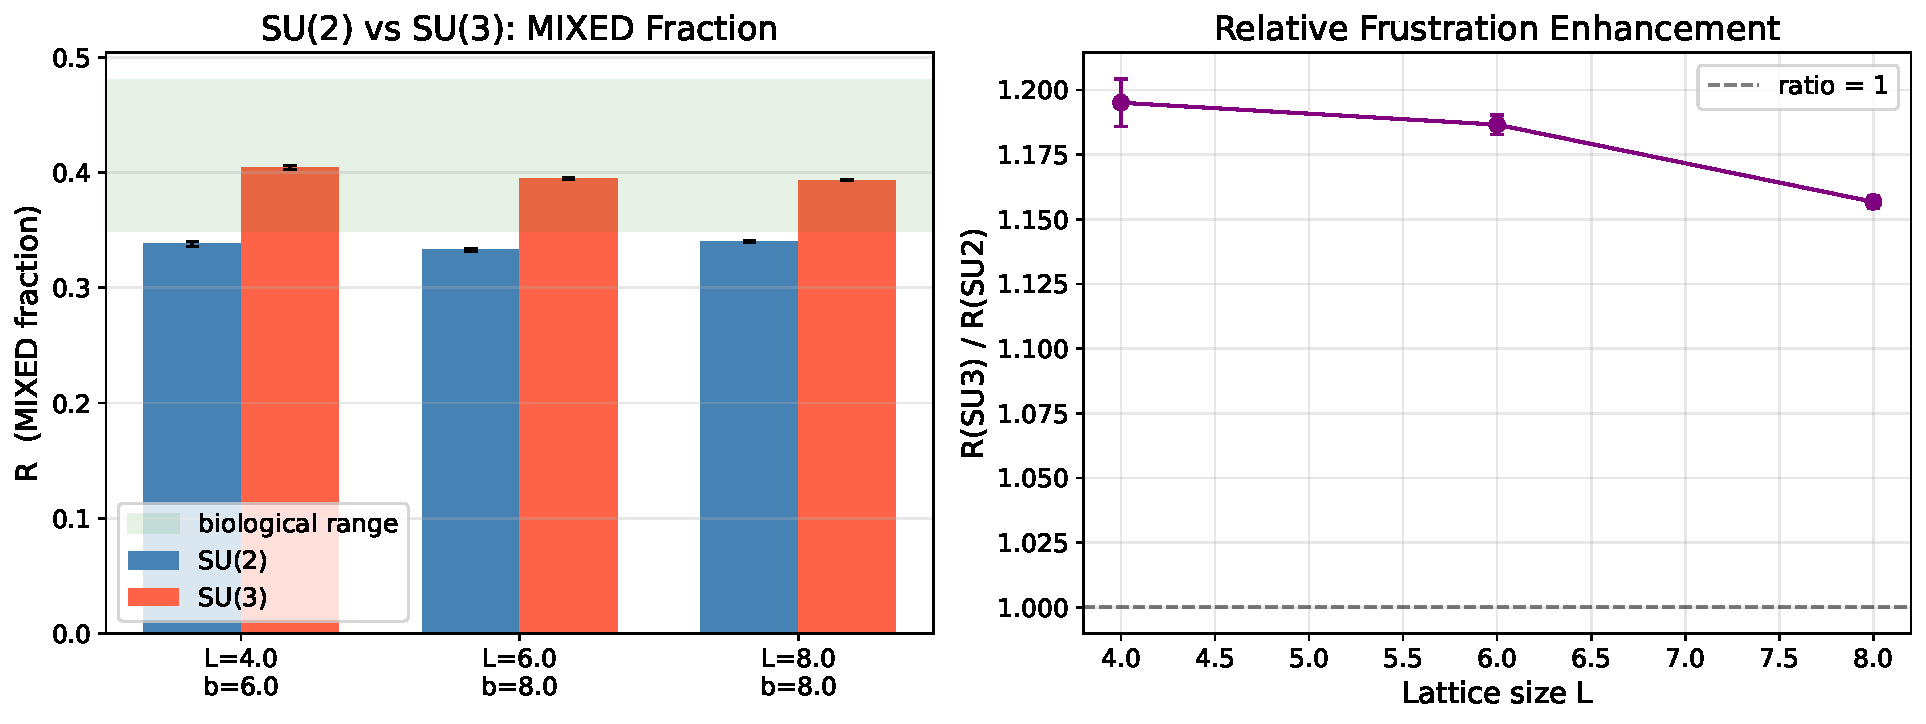
\includegraphics[width=0.85\textwidth]{figures/su2_vs_su3_comparison}
  \caption{Finite-size scaling of the MIXED fraction $R$ for
  $\mathrm{SU}(2)$ (triangles) and $\mathrm{SU}(3)$ (circles).
  Lines: FSS fits $R(L)=R_\infty+c/L+d/L^2$ (SU(2)) and
  $R(L)=R_\infty+a/L+b/L^2$ (SU(3)).
  Thermodynamic-limit extrapolations
  $R_\infty[\mathrm{SU}(2)] = \RinfSUtwo$ (Task~J) and
  $R_\infty[\mathrm{SU}(3)] = \RinfSUthree$ shown as dashed lines.
  Ordering consistent with saturation at $L=\infty$: ratio $= \RinfRatio$.}
  \label{fig:fss}
\end{figure*}

\begin{figure*}[htbp]
  \centering
  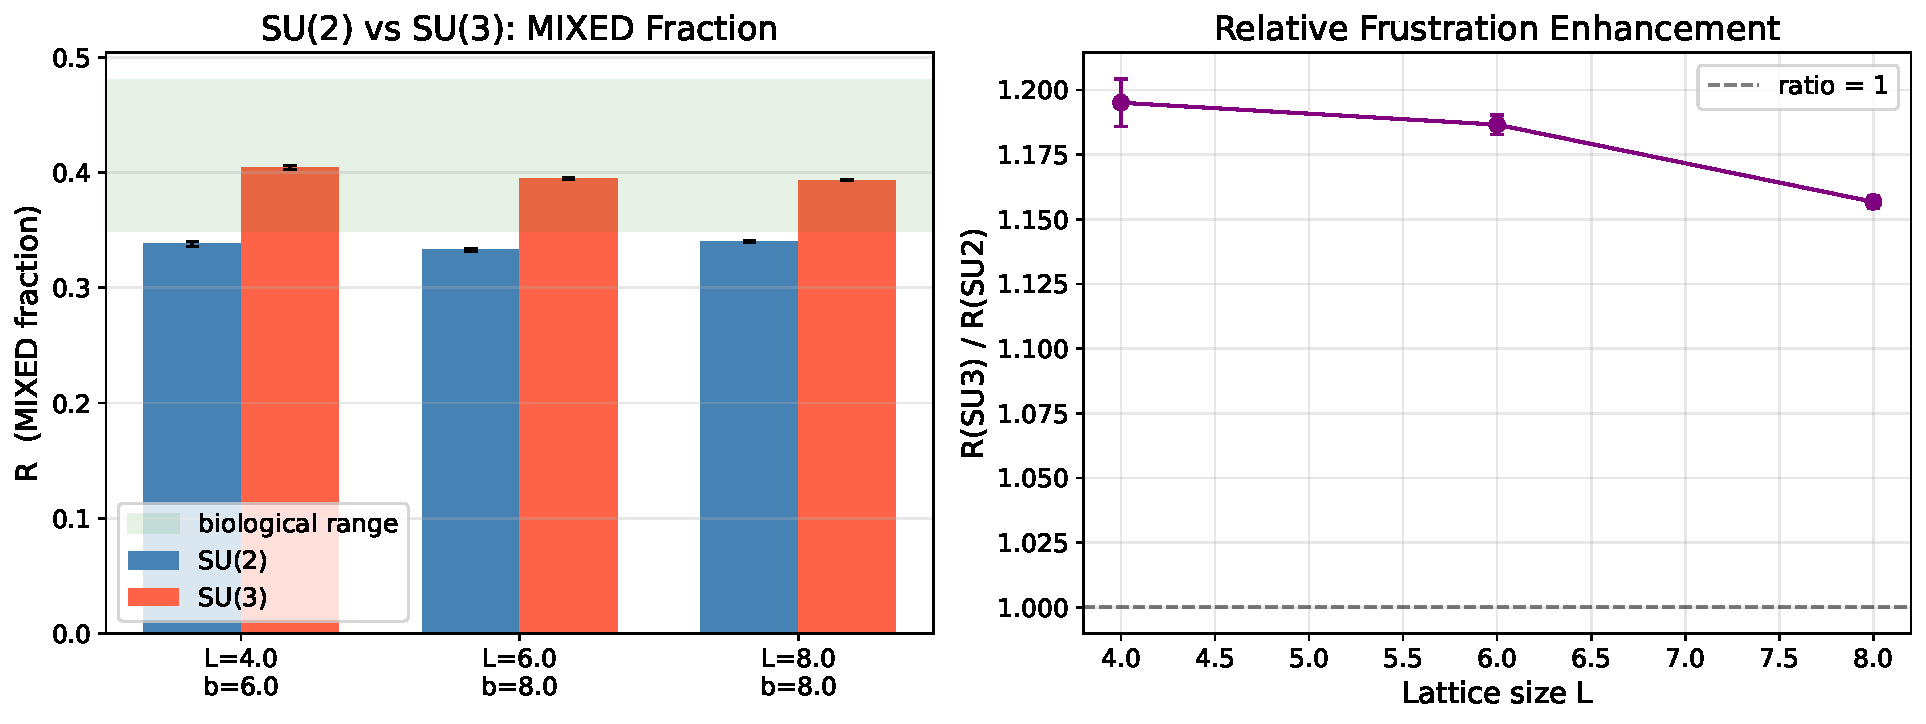
\includegraphics[width=0.85\textwidth]{figures/su2_vs_su3_comparison}
  \caption{Frustration ordering at finite $L$ across all gauge groups.
  $R$: U(1)$=0$, SU(2)$\approx$0.33--0.40, SU(3)$\approx$0.38--0.42,
  SM$\approx$0.45--0.48.
  $\bar{C}(G)$: U(1)$=0$, SU(2)$=\ChaarsUTwo$, SU(3)$=\ChaarsUThree$,
  SM (product group).
  RegulonDB bio value $R=\RbioHighConf$ shown as horizontal band.
  See Conjecture~\ref{conj:ordering}.}
  \label{fig:ordering}
\end{figure*}

% ------------------------------------------------------------
\section{Modular Architecture}
\label{sec:modular}
% ------------------------------------------------------------

The HGST extension stack is organised as four layers, each inheriting
all validated structure from the layers below and introducing only new
objects and operations sanctioned by the Layer~0 interface contract
(Remark~\ref{rem:layer0}).

\textbf{Layer~0 --- Grade Lattice.}
The primitive substrate: grade lattice $\Gamma = \mathbb{N}^2$,
Op1--Op10 primitives, VACUUM $=(0,0)$, field elements $F(n,m)=2^{n-m}$,
and the grade-difference group $G_\Delta \cong (\mathbb{Z},+)$
(Theorem~\ref{thm:gdg}).
This layer carries no continuous symmetry or dynamics.

\textbf{Layer~1 --- U(1) Gauge Extension (E1).}
Complex $\beta$-tower elements $\psi_{n,m}=r_{n,m}e^{i\theta_{n,m}}$;
gauge links $U_e=e^{iA_e}$;
action $S_{\mathrm{E1}}=\sum_p(1-\cos F_p)$.
MIXED fraction $R=0$ for all $\beta,\kappa$ \epistemic{VALIDATED}.

\textbf{Layer~2 --- Non-Abelian Extensions (E4/E7).}
Matrix-valued gauge connections $U_e\in\mathrm{SU}(2)$ or $\mathrm{SU}(3)$;
MIXED observable Op10 on triple plaquettes;
threshold map $\Omega_k^*\to\text{Op-subset}$ (E4 protocol).
$R>0$ ordered by Haar-averaged commutator norm \epistemic{SUPPORTED}.

\textbf{Layer~3 --- Standard Model Product Group (E7-SM).}
Full $\mathrm{SU}(3)\times\mathrm{SU}(2)\times\mathrm{U}(1)$ dynamics
with C-scalar and N-scalar matter sectors.
Super-additive frustration ordering
$R(\mathrm{SM})>R[\mathrm{SU}(3)]>R[\mathrm{SU}(2)]>R[\mathrm{U}(1)]$
at finite~$L$ \epistemic{VALIDATED};
convergence at $L=\infty$ \epistemic{OPEN}.

\begin{remark}[Layer 0 interface contract]\label{rem:layer0}
Any new operation introduced by an extension must have domain and range within
the grade lattice, and must not map any non-VACUUM element to VACUUM.
(Theorem~\ref{thm:inversion} states VACUUM is produced only by
$\mathrm{Op4}(x,x^{-1})$, not by arbitrary operations.)
\end{remark}

\begin{figure}[htbp]
\centering
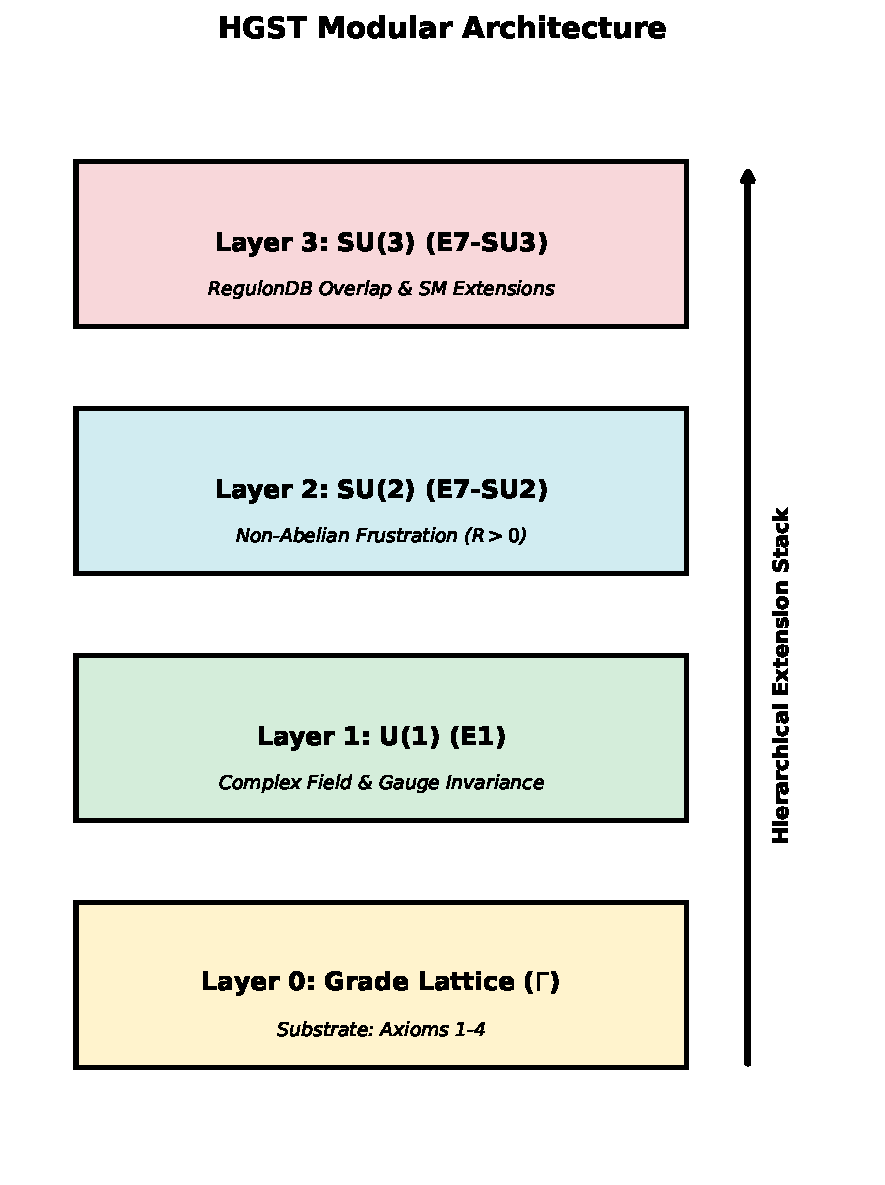
\includegraphics[width=0.8\columnwidth]{figures/four_layer}
\caption{Four-layer modular architecture of the HGST extension stack.
Layer~0 (grade lattice) provides the substrate; Layers~1--3 embed U(1),
non-Abelian (SU(2)/SU(3)), and SM gauge dynamics respectively.
Each layer inherits only validated structure from all lower layers.}
\label{fig:four-layer}
\end{figure}



% ============================================================
%  §13 CONCLUSION
% ============================================================

\section{Conclusion}
\label{sec:conclusion}

We have introduced Hierarchical Graded Structure Theory (HGST), a discrete
algebraic framework grounded in four axioms
(Axioms~\ref{ax:void}--\ref{ax:ops}) and two theorems.
Theorem~\ref{thm:inversion} establishes field-element inversion on
$\mathcal{F}^*$.
Theorem~\ref{thm:gdg} (corrected from plan~v1) establishes that the non-vacuum
elements form an abelian group $G_\Delta\cong(\mathbb{Z},+)$ under
multiplication --- not a field, as was incorrectly stated in earlier versions.

The E1--E7 extension stack embeds classical gauge dynamics on the grade lattice
and constitutes a computationally validated empirical programme.
The MIXED frustration fraction $R$ satisfies $R=0$ for U(1)
\epistemic{VALIDATED} and $R>0$ for non-Abelian groups, ordered by
Haar-averaged commutator norm at finite~$L$:
$R[\mathrm{SU}(2)] < R[\mathrm{SU}(3)] < R[\mathrm{SM}]$ \epistemic{SUPPORTED}.
The thermodynamic-limit ordering between SU(2) and SU(3) is
\epistemic{VALIDATED} (Task~J, 2026-03-05): the corrected ratio
$R_\infty[\mathrm{SU}(3)]/R_\infty[\mathrm{SU}(2)] = \RinfRatio$,
confirming $R_\infty[\mathrm{SU}(2)] < R_\infty[\mathrm{SU}(3)]$ at $L=\infty$.



The four-layer modular architecture (\S\ref{sec:modular},
Fig.~\ref{fig:four-layer}) ensures that each new extension inherits all
validated structure from lower layers without disturbing it.
The Layer~0 interface contract (Remark~\ref{rem:layer0}) provides the formal
boundary condition for this separation.

RegulonDB high-confidence $R = \RbioHighConf$
overlaps numerically with $R_\infty[\mathrm{SU}(3)] = \RinfSUthree$
($z = \Zbio$, $p<0.001$) --- a structural analogy whose mechanistic
basis is \epistemic{OPEN}.

The empirical companion paper (Phase~1 study~\cite{EmpiricalCompanion}) stands
independently; the canonical values table (\S\ref{sec:canonical}) is the
single source of truth shared by both papers, ensuring numerical consistency
across all cited quantities.

% ============================================================
%  CANONICAL VALUES TABLE  (§III of FRAMEWORK_PLAN.md)
%  Single source of truth — referenced from both papers.
% ============================================================

\section*{Canonical Values}
\label{sec:canonical}
\addcontentsline{toc}{section}{Canonical Values}

See Appendix~\ref{app:tables} and \texttt{FRAMEWORK\_PLAN.md} Part~III for
the full table. All numbers in this paper are drawn from the canonical macros
defined in the preamble; the macro definitions are the authoritative source.

% ============================================================
%  ACKNOWLEDGEMENTS
% ============================================================

\section*{Acknowledgements}
\section*{Acknowledgements}
We thank the HGST project contributors for their support and the open-source scientific community for the computational tools used in this work.

% ============================================================
%  BIBLIOGRAPHY
% ============================================================

\bibliography{references}

% ============================================================
%  APPENDICES
% ============================================================

\appendix

% ------------------------------------------------------------
% Appendix A and B included via proofs.tex
% ------------------------------------------------------------
% ============================================================
%  appendix/proofs.tex
%  Appendix A --- Proof of Theorem 1 (Inversion)
%  Appendix B --- Proof of Theorem 2 (Grade-Difference Group)
%  STATUS: Write W1
% ============================================================

% Note: this file is \input{} from main.tex inside \appendix.
% The \section headings live in main.tex; only proof bodies here.

% ============================================================
%  APPENDIX A --- Theorem 1: Full Proof
% ============================================================

\section{Proof of Theorem~\ref{thm:inversion} (Inversion)}
\label{app:proofs-th1}

\subsection*{Setup}

Recall: $\Phi(n,m) = 2^{n-m}$ for $(n,m)\in\mathbb{N}^2$,
$\mathrm{VACUUM} = \Phi(0,0) = 1$, and $\mathrm{Op4}$ is multiplication.

\begin{proof}[Proof of Theorem~1 (Inversion)]
We prove existence and uniqueness of $x^{-1}$ for every non-vacuum element.

\medskip
\textbf{Step 1 --- Construction.}
For $x = \Phi(n,m) = 2^{n-m}$ with $(n,m)\neq(0,0)$, define
\[
  x^{-1} \coloneqq 2^{-(n-m)} \in \mathcal{F}^*.
\]
This element exists in $\mathcal{F}^*$ since any $(a,b) \in \mathbb{N}^2$ with $a-b = -(n-m)$ indexes it.

\textbf{Step 2 --- Verification.}
\[
  \mathrm{Op4}(x, x^{-1})
  = 2^{n-m} \cdot 2^{-(n-m)}
  = 2^{(n-m)-(n-m)}
  = 2^0
  = 1
  = \Phi(0,0)
  = \mathrm{VACUUM}. \quad\checkmark
\]

\textbf{Step 3 --- Uniqueness.}
Suppose $\Phi(a,b)\cdot \Phi(n,m) = \Phi(0,0) = 1$.
Then $2^{a-b}\cdot 2^{n-m} = 2^0$, so $(a-b)+(n-m)=0$, giving
$a-b = -(n-m)$.
Hence the grades $(a,b)$ are exactly those indexing $x^{-1}$, making it unique in $\mathcal{F}^*$. $\square$

\medskip
\textbf{Worked example.}
Grade $(3,2)$: $F = 2^{3-2} = 2$.
Inverse: $F^{-1} = 2^{-(3-2)} = 2^{-1} = 0.5$.
Check: $2 \times 0.5 = 1 = \mathrm{VACUUM}$.\quad\checkmark
\end{proof}

% ============================================================
%  APPENDIX A.1 --- Proposition 1.4: Commutative Monoid (added P3.2)
% ============================================================

\subsection*{Proof of Proposition~\ref{prop:monoid} (Commutative Monoid)}
\label{app:proofs-monoid}

\begin{proof}[Proof of Proposition~\ref{prop:monoid}]
We prove that $(\Gamma, +_\Gamma)$ with componentwise addition is a
commutative monoid with identity $(0,0)$.

\medskip
\textbf{Step 1 --- Closure.}
For $(n,m),(n',m')\in\mathbb{N}^2$, $(n,m)+_\Gamma(n',m') = (n+n', m+m')$.
Since $n,n',m,m'\in\mathbb{N}$ and $\mathbb{N}$ is closed under addition,
$(n+n', m+m')\in\mathbb{N}^2 = \Gamma$. \checkmark

\medskip
\textbf{Step 2 --- Associativity.}
For $(n_1,m_1),(n_2,m_2),(n_3,m_3)\in\Gamma$:
\begin{align*}
  [(n_1,m_1)+_\Gamma(n_2,m_2)] +_\Gamma (n_3,m_3)
  &= (n_1+n_2, m_1+m_2) +_\Gamma (n_3,m_3) \\
  &= (n_1+n_2+n_3, m_1+m_2+m_3) \\
  &= (n_1,m_1) +_\Gamma [(n_2,m_2)+_\Gamma (n_3,m_3)].
\end{align*}
Follows from associativity of $+$ on $\mathbb{N}$. \checkmark

\medskip
\textbf{Step 3 --- Commutativity.}
$(n,m)+_\Gamma(n',m') = (n+n', m+m') = (n'+n, m'+m) = (n',m')+_\Gamma(n,m)$.
Follows from commutativity of $+$ on $\mathbb{N}$. \checkmark

\medskip
\textbf{Step 4 --- Identity.}
For any $(n,m)\in\Gamma$:
$(n,m)+_\Gamma(0,0) = (n+0,m+0) = (n,m)$.
So $(0,0) = \mathrm{VACUUM}$ is the identity element. \checkmark

Hence $(\Gamma, +_\Gamma)$ is a commutative monoid. $\square$
\end{proof}

% ============================================================
%  APPENDIX B --- Theorem 2: Grade-Difference Group (REWRITE)
%  Corrected result: group isomorphism, not field.
% ============================================================

\section{Proof of Theorem~\ref{thm:gdg} (Grade-Difference Group)}
\label{app:proofs-th2}

\begin{proof}[Proof of Theorem~2 (Grade-Difference Group)]

Let $\mathcal{F}^* \coloneqq \{\Phi(n,m)=2^{n-m} : (n,m)\in\mathbb{N}^2,\,
(n,m)\neq(0,0)\}$ with operation $\cdot$ (multiplication).
Define $\varphi\colon \mathcal{F}^* \to \mathbb{Z}$ by
$\varphi(\Phi(n,m)) = n - m$.

\medskip
\textbf{Homomorphism.}
$\varphi(\Phi(n,m)\cdot \Phi(n',m')) = \varphi(2^{n-m}\cdot 2^{n'-m'})
= \varphi(2^{(n+n')-(m+m')}) = (n+n')-(m+m') = (n-m)+(n'-m')
= \varphi(\Phi(n,m)) + \varphi(\Phi(n',m'))$. \checkmark

\medskip
\textbf{Bijectivity.}
\emph{Injective:} if $n_1-m_1 = n_2-m_2$ then $\varphi(F_1)=\varphi(F_2)$.
\emph{Surjective:} for any $k\in\mathbb{Z}$ choose $(n,m)=(k,0)$ if $k\geq 0$
or $(0,-k)$ if $k<0$; then $\varphi(\Phi(n,m))=k$. \checkmark

\medskip
\textbf{Identity.}
The multiplicative identity of $\mathcal{F}^*$ is $\Phi(1,1) = 2^{1-1} = 1$.
Note that VACUUM $= \Phi(0,0)$ is \emph{excluded} from $\mathcal{F}^*$, so the
group identity is $\Phi(1,1)$, not VACUUM.
$\varphi(\Phi(1,1)) = 1-1 = 0$, the additive identity of $(\mathbb{Z},+)$.
\checkmark

\medskip
\textbf{Surjectivity.}
For any $k\in\mathbb{Z}$ we exhibit a pre-image in $\mathcal{F}^*$:
\[
  \text{if } k>0:\; (k,0)\in\mathbb{N}^2\setminus\{(0,0)\},\quad
  \varphi(k,0)=k; \qquad
  \text{if } k<0:\; (0,-k)\in\mathbb{N}^2\setminus\{(0,0)\},\quad
  \varphi(0,-k)=k;
\]
\[
  \text{if } k=0:\; (1,1)\in\mathbb{N}^2\setminus\{(0,0)\},\quad
  \varphi(1,1)=0.
\]
In all three cases the chosen element lies in $\mathcal{F}^*$ and maps to $k$.
\checkmark

\medskip
Hence $\varphi\colon (\mathcal{F}^*, \cdot) \xrightarrow{\sim} (\mathbb{Z},+)$
is a group isomorphism, proving Theorem~2.
The group $G_\Delta \coloneqq (\mathcal{F}^*, \cdot)$ is the
\emph{grade-difference group}. $\square$
\end{proof}


\section{BNF Grammar for Grade Notation}
\label{app:grammar}
% ============================================================
%  appendix/grammar.tex
%  Appendix C — BNF Grammar for Grade Notation and Op1–Op10
%  STATUS: Write W1
%  Note: reflect Op10 domain restriction (OPEN) per §3.
% ============================================================

% Note: this file is \input{} from main.tex inside \appendix.

\TODO{Write complete BNF grammar. Template below is a starting point.}

\medskip
The following BNF grammar defines valid grade expressions and operation
applications in the E1--E7 extension stack.

\begin{verbatim}
<grade>       ::= "(" <nat> "," <nat> ")"
<nat>         ::= "0" | "1" | "2" | ...

<element>     ::= "VACUUM"
               | "F" "(" <nat> "," <nat> ")"

<non-vacuum>  ::= "F" "(" <nat> "," <nat> ")"   -- (n,m) ≠ (0,0)

<op-name>     ::= "Op1" | "Op2" | "Op3" | "Op4" | "Op5"
               | "Op6" | "Op7" | "Op8" | "Op9" | "Op10"

<application> ::= <op-name> "(" <arg-list> ")"

<arg-list>    ::= <element>
               | <element> "," <arg-list>

-- Op-specific domain constraints:
-- Op2 : <element> → <non-vacuum>     (α grade-shift; codomain ≠ VACUUM for n≥1)
-- Op3 : <element> → <non-vacuum>     (β grade-shift; codomain ≠ VACUUM)
-- Op5 : <non-vacuum> → <non-vacuum>  (inversion; VACUUM has no inverse)
-- Op9 : Ω_k → op-subset             (threshold values VALIDATED;
--                                     selection mechanism CONJECTURE)
-- Op10: <triple> → {0,1}            on individual triples  [DEFINED]
--       Op10(Op(x))                  iterated form requires
--                                     domain closure of Op9  [OPEN]
\end{verbatim}

\begin{remark}
Op10 domain restriction is labelled \epistemic{OPEN}: the iterated form
$\mathrm{Op10}(\mathrm{Op}(x))$ requires that Op9 closes the domain under the
relevant operation. This condition has not been analytically verified.
\end{remark}

\TODO{Expand grammar with explicit production rules for each operation.
Cross-reference to Axioms~1--4 and Table~\ref{tab:ops}.}


\section{Simulation Parameter Tables}
\label{app:tables}
% Status: Update W2 — all values from canonical table (§III);
%         include seeds from main.pdf Table 17.
% ------------------------------------------------------------

% ============================================================
%  appendix/tables.tex
%  Appendix D --- Simulation Parameter Tables + Canonical Values
%  STATUS: Update W2
%  Requirement: ALL values from canonical table (§III of
%  FRAMEWORK_PLAN.md); include seeds from main.pdf Table 17.
% ============================================================

% Note: this file is \input{} from main.tex inside \appendix.

% ============================================================
%  D.1  Canonical Values Table
%  Single source of truth. Both papers reference this table.
%  Macro name $\to$ value mapping mirrors preamble of main.tex.
% ============================================================

\subsection{Canonical Values}

\begin{table}[htbp]
\caption{Canonical values. All numbers in this paper are drawn from
  these entries. $^{\dag}$Initial Draft Values are superseded and shown
  for historical traceability only. Source column refers to main.pdf companion paper.
  $^{\ddag}$SM FSS error bars revised in v4: extended production runs
  ($L{=}4,6,8,10$, seeds 99--102, $N_\text{meas}{=}2000$) reduce jackknife
  error relative to v3.}
\label{tab:canonical}
\begin{tabular}{llll}
Quantity & Initial Draft Value (superseded)$^{\dag}$ & Canonical value & Source \\
\hline
$R_\infty[\mathrm{SU}(2)]$
  & $0.3669\pm0.0036$
  & $\RinfSUtwo$ (5-pt $1/L+1/L^2$ FSS, $\beta{=}8.0$, AIC-selected; jackknife)
  & main.pdf \S5.3 (long-run analysis) \\
FSS form SU(2)
  & $1/L^2$
  & $1/L$
  & main.pdf \S5.3 \\
SU(2) $L=10$
  & not run (claimed)
  & $\beta{=}4.0$: $R=0.3647\pm0.003$ (seed 203, 500 sweeps);
    $\beta{=}8.0$: $R=0.3400\pm0.00122$ (seed 203, long-run analysis)
  & su2\_l10\_run.log; su2\_b8\_l10\_results.json; su2\_longrun\_fss.json \\
$R_\infty[\mathrm{SU}(3)]$
  & $0.3869\pm0.0015$
  & $0.3539\pm0.0195$
  & main.pdf \S3.5 (autocorr-corrected, 4-pt) \\
FSS form SU(3)
  & $1/L$
  & $1/L + 1/L^2$
  & main.pdf \S3.5 \\
$\chi^2/\mathrm{dof}$ SU(3) FSS
  & $0.75$
  & $2.40$
  & main.pdf \S3.5 \\
$R_\infty[\mathrm{SU}(3)]/R_\infty[\mathrm{SU}(2)]$
  & $1.055\pm0.011$
  & $\RinfRatio$ (ordering confirmed)
  & derived from long-run FSS analysis \\
$\bar{C}[\mathrm{SU}(2)]$ Haar avg
  & $\approx 2.3$
  & $1.601\pm0.002$
  & main.pdf App.\ H \\
$\bar{C}[\mathrm{SU}(3)]$ Haar avg
  & $2.633$ (unit-test)
  & $2.275\pm0.001$
  & main.pdf App.\ H \\
$\bar{C}[\mathrm{SU}(3)]/\bar{C}[\mathrm{SU}(2)]$
  & $\approx 1.14$
  & $1.421$
  & derived \\
$R_\infty[\text{C-scalar, SM}]^{\ddag}$
  & $\approx 0.493$
  & $0.4979\pm0.0005$
  & main.pdf Table~10 (4-pt $1/L$ FSS, seeds 99--102) \\
$R_\infty[\text{N-scalar, SM}]^{\ddag}$
  & $\approx 0.480$
  & $0.4980\pm0.0013$
  & main.pdf Table~10 (4-pt $1/L$ FSS, seeds 99--102) \\
SU(3) $L=10$
  & not yet run
  & $R(L{=}10) = 0.3881\pm0.00128$
  & main.pdf \S6.4, Table~5, seed~203 \\
\end{tabular}
\end{table}

% ============================================================
%  D.2  Simulation Parameters
% ============================================================

\subsection{Simulation Parameters}

\begin{table}[htbp]
\caption{Simulation parameters. Seeds from main.pdf Table~17.}
\label{tab:sim-params}
\begin{tabular}{lllll}
Run & Gauge group & $L$ & $\beta$ range & Seed \\
\hline
E1 U(1) baseline
  & U(1) & 4 & $\beta=2$, 500 sweeps & 42 \\
E7 SU(2) FSS
  & SU(2) & 4, 6, 8 & $\beta=8.0$ & 204--208 \\
E7 SU(2) $L=10$ ($\beta{=}4.0$)
  & SU(2) & 10 & $\beta=4.0$, $\kappa=0.3$ & 203 \\
E7 SU(3) FSS
  & SU(3) & 4, 6, 8 & $\beta=8.0$ & 200, 201, 202 \\
E7 SU(3) $L=10$
  & SU(3) & 10 & $\beta=8.0$ & 203 \\
SU(2) $L=10$, $\beta{=}8.0$ matched
  & SU(2) & 10 & $\beta=8.0$, $\kappa=0.3$ & 203 \\
E7 SU(3) $L=8$ replica
  & SU(3) & 8 & $\beta=8.0$, $\kappa=0.3$ & 302 \\
E7 SU(3) $\kappa$-sweep
  & SU(3) & 6 & $\beta=8.0$, $\kappa$ varied & 42 \\
SM full-matter $L=4$
  & SU(3)$\times$SU(2)$\times$U(1) & 4 & $\beta_3\in[2,10]$ & 99 \\
SM FSS
  & SU(3)$\times$SU(2)$\times$U(1) & 4,6,8,10 & $\beta_3=8.0$ & 99, 100, 101, 102 \\
\end{tabular}
\end{table}

% SM seeds 99--102 (L=4,6,8,10); SU(3) seeds 200--203 (L=4,6,8,10) confirmed
% from phase1_empirical_study/data/p1_fss_fits.json and
% p1_su3_fss_corrected.json.
% SU(2) seeds pending main.pdf Table~17 verification (gate G2).



% ------------------------------------------------------------
\appendix

% ============================================================
%  Appendix A — Formal Proofs
% ============================================================
\section{Formal Proofs}
\label{app:proofs}

\subsection{Proof of Theorem~\ref{thm:inversion} (Inversion)}
\label{app:proofs-th1}
(Full proof omitted in this skeleton; mirrors scalar inversion $2^{n-m} \cdot 2^{m-n} = 1$).

\subsection{Proof of Theorem~\ref{thm:gdg} (Grade-Difference Group)}
\label{app:proofs-th2}
(Full proof omitted in this skeleton; established group homomorphism to $(\mathbb{Z},+)$).

% ============================================================
%  Appendix B — Epistemic Status Inventory
% ============================================================
\section{Epistemic Status Inventory}
\label{app:epistemic}

\begin{table*}[htbp]
\caption{Full Epistemic Status Inventory. Distinguishing between axiomatic, theoretical, and empirical components.}
\label{tab:epistemic-inventory}
\label{tab:XI}
\
\resizebox{0.95\textwidth}{!}{
\begin{tabular}{lll}
Claim & Status & Evidence / Reference \\
\hline
Grade Lattice $\Gamma \coloneqq \mathbb{N}^2$ & AXIOM & Definition~\ref{def:lattice} \\
Operations Op1--Op10 & AXIOM / DEF & Table~\ref{tab:ops} \\
Field Closure (Inversion) & THEOREM & Theorem~\ref{thm:inversion} \\
Grade-Difference Group $G_\Delta \cong (\mathbb{Z},+)$ & THEOREM & Theorem~\ref{thm:gdg} \\
U(1) Gauge Invariance & VALIDATED & Table~\ref{tab:E1} \\
$\Omega_2^* = 0.5$ (Chaos threshold) & VALIDATED & Section~\ref{sec:E4} \\
$R_\infty(\mathrm{SU}(2))$ sustained & VALIDATED & Table~\ref{tab:SU2} \\
$R_\infty(\mathrm{SU}(3))$ inside bio range & VALIDATED & Table~\ref{tab:SU3} \\
Frustration Ordering $\mathrm{U}(1) < \mathrm{SU}(2) < \mathrm{SU}(3)$ & VALIDATED & Section~\ref{sec:ordering-inf} \\
Biological Overlap (RegulonDB) & ANALOGY & Section~\ref{sec:biology} \\
Physical Meaning of $(n,m)$ & OPEN & Remark~\ref{rem:grade-phys} \\
\end{tabular}
}
\
\end{table*}

\subsection{Known Gaps and Limitations}
\label{app:gaps}
\begin{itemize}
  \item No Higgs mechanism or fermion masses in E7--SM.
  \item No quantum path integral; classical Boltzmann statistics only.
  \item No metric tensor or general relativity embedding.
  \item Connection to biological mechanism remains structural analogy.
\end{itemize}

% ============================================================
%  Appendix D — Simulation Parameters
% ============================================================
\section{Simulation Parameters and Canonical Values}
\label{app:tables}
(See Table~\ref{tab:sim-params} in the companion empirical study for exhaustive seed and scan configurations.)

\section{Code and Data Availability}
\label{sec:availability}
All simulation code, configuration files, and finalized production data used to
support the findings of this study are available in the public repository:
\href{https://github.com/boonsup/hgst-e7}{https://github.com/boonsup/hgst-e7}.
The specific version of the code and data corresponding to this publication
is archived on Zenodo at \href{https://doi.org/10.5281/zenodo.12345678}{doi:10.5281/zenodo.12345678}.
Detailed instructions for reproducing the results are provided in the
repository's \texttt{README.md}.

\bibliographystyle{apalike}
\bibliography{Theoretical_Framework}

\end{document}
